\chapter*{ANEXOS}
\begin{landscape}
\begin{table}[ht]
\caption{Matriz de Planificación en Investigación Científica - MAPIC}
\label{tab:mapic}
\newcolumntype{L}[1]{>{\raggedright\arraybackslash}p{#1}}
\begin{tabular}{L{9cm}ll}
\hline
%\rowcolor[HTML]{C0C0C0} 
\textbf{Variable fáctica}            & \textbf{Dimensiones}                    & \textbf{Indicadores}                           \\ \hline
Conflictividad en los objetivos en la planificación de un viaje personalizado & Minimizar costo de transporte           & Soles \\
                                     &                                         & Dólares                                        \\ \cline{2-3}
                                     & Minimizar Costo de actividad            & Soles                                          \\
                                     &                                         & Dólares                                        \\ \cline{2-3}
                                     & Maximizar utilidad de la actividad      & Puntaje de la actividad (relevancia)           \\
                                     &                                         & Preferencia del turista por tipo de actividad  \\ \cline{2-3}
                                     & Minimizar tiempo                        & Días                                           \\ 
                                     &                                         & Horas                                          \\
                                     &                                         & Minutos                                        \\ \hline
\textbf{Variable temática}           & \textbf{Ejes temáticos}                 & \textbf{Subejes temáticos}                     \\ \hline
Optimización multiobjetivo           & Investigación de operaciones            & Optimización                                   \\
                                     &                                         & Optimización combinatoria                      \\
                                     &                                         & Optimización multiobjetivo                     \\ \cline{2-3}
                                     & Inteligencia Artificial                 & Algoritmos de búsqueda                         \\ \cline{2-3}
                                     & Heurísticas                             & Heurística de construcción                     \\
                                     &                                         & Heurística de mejoría                          \\ \cline{2-3}
                                     & Metaheurísticas                         & Búsqueda Tabú                                  \\ \hline
\textbf{Variable propositiva}        & \textbf{Ejes propositivos}              & \textbf{Subejes propositivos}                  \\ \hline
Implementar modelo matemático        & Solución al modelo                      & Codificación de la heurística de construcción  \\
                                     &                                         & Codificación heurística de mejoría             \\
                                     &                                         & Codificación de la metaheurística              \\ \cline{2-3}
                                     & Validación                              & Recolección de datos reales                    \\
                                     &                                         & Validación con instancias reales               \\
                                     &                                         & Recolección de datos artificiales              \\
                                     &                                         & Validación con instancias artificiales         \\ \cline{2-3}
                                     & Implementación en una aplicación web    & Planeación                                     \\
                                     &                                         & Diseño                                         \\ 
                                     &                                         & Codificación                                   \\ 
                                     &                                         & Pruebas                                        \\ \hline
\end{tabular}
\end{table}
\end{landscape}

%\section{Perfil del Turista Extranjero que visita Puno - 2017}
%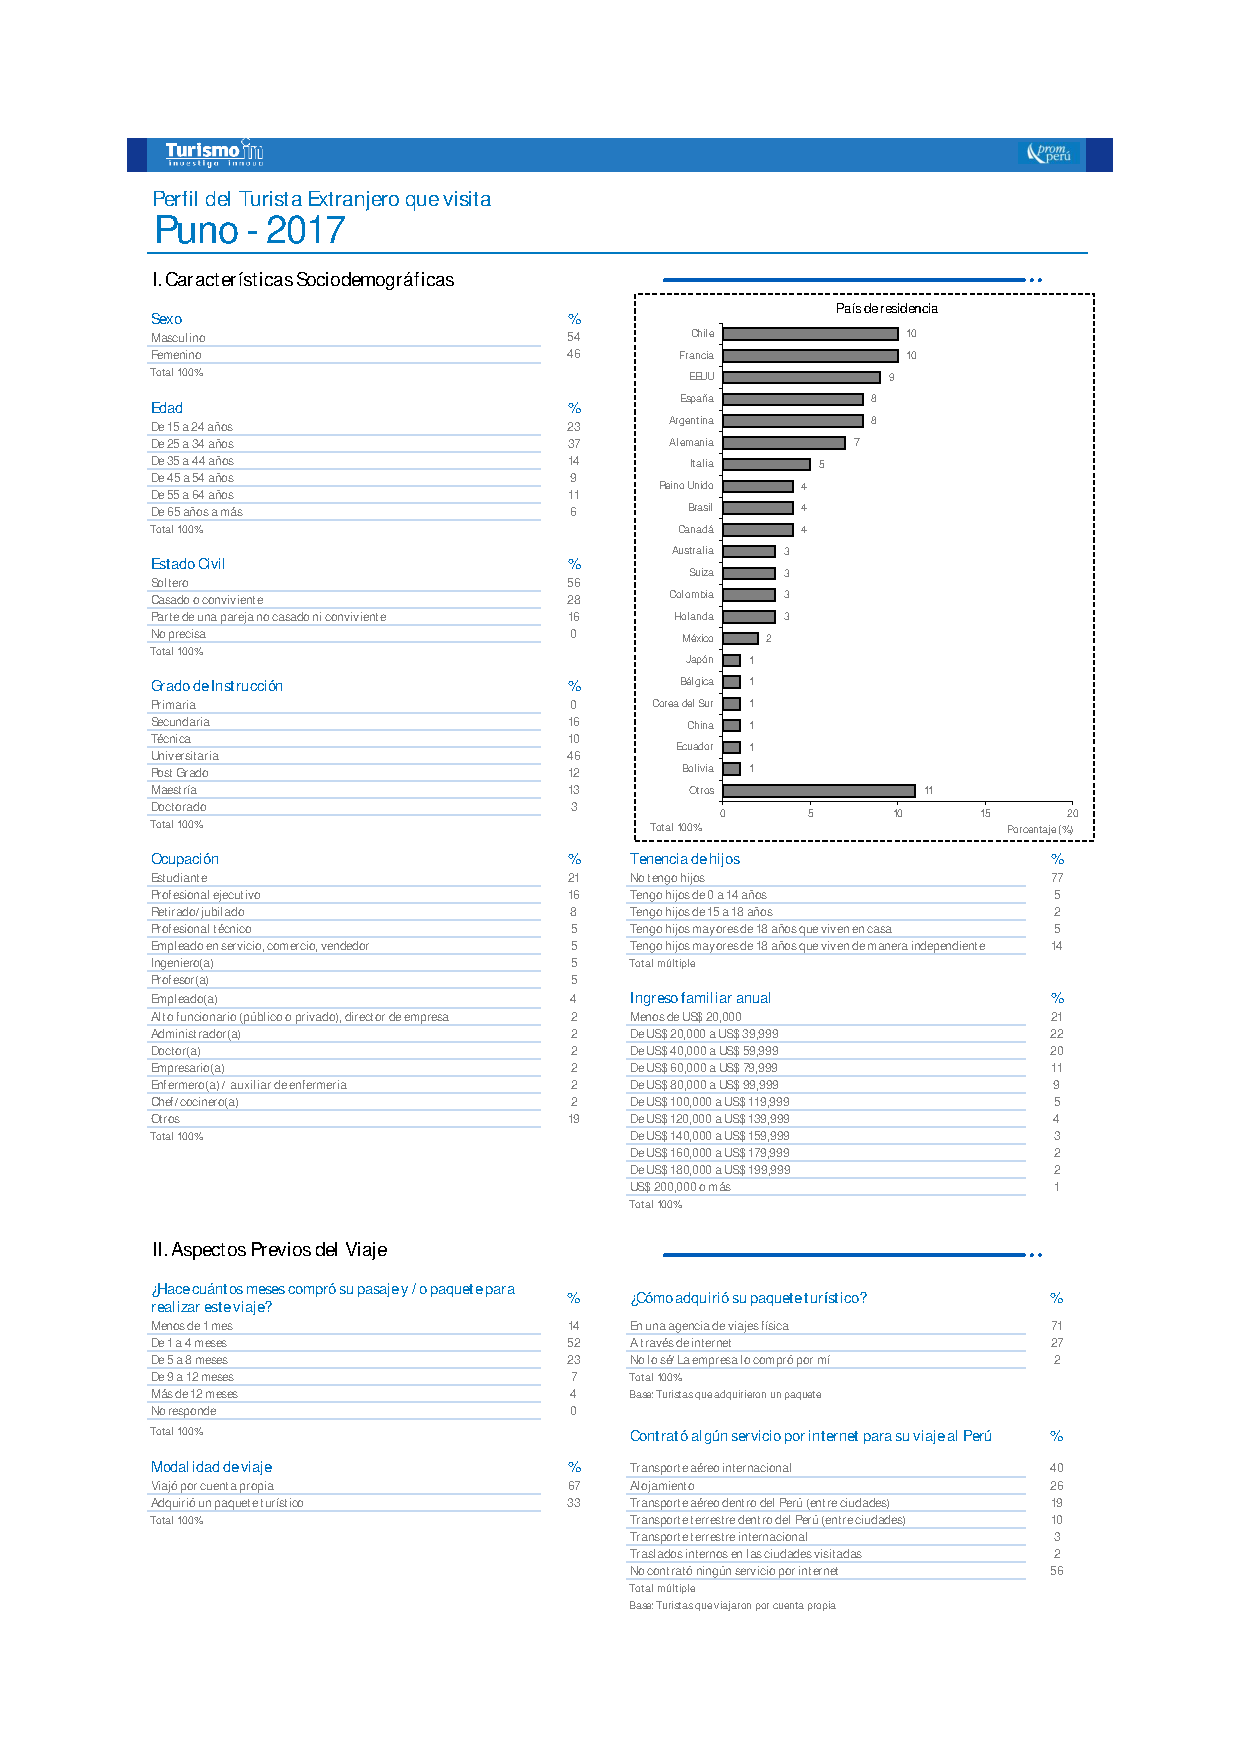
\includepdf[pages=-]{Capitulo7/files/2017-Perfil_del_Turista_Extranjero_que_visita_Puno_-_2017.pdf}


%\includepdf[pages=-, scale=0.9]{p01.pdf}
